\chapter{基于FLUENT软件的轴承静态特性研究}

% 1. 插图: 图应有自明性。插图应与文字紧密配合，文图相符，内容正确。选图要力求精练，插图、照片应完整清晰。图中文字和数字等字号用宋体5号字。
% 机械工程图：采用第一角投影法，严格按照GB4457～GB131-83《机械制图》标准规定。
% 数据流程图、程序流程图、系统流程图等按GB1526-89标准规定。
% 电气图：图形符号、文字符号等应符合附录3所列有关标准的规定。
% 流程图：必须采用结构化程序并正确运用流程框图。
% 对无规定符号的图形应采用该行业的常用画法。
% 坐标图的坐标线均用细实线，粗细不得超过图中曲线，有数字标注的坐标图，必须注明坐标单位。
% 照片图要求主题和主要显示部分的轮廓鲜明，便于制版。如用放大或缩小的复制品，必须清晰，反差适中。照片上应有表示目的物尺寸的标度。引用文献图表必须标注出处。

% 2. 图题及图中说明: 每个图均应有图题（由图序和图名组成），图名在图序之后空一格排写。图序按章编排，如第1章第一个插图的图号为“图1-1”等。图题置于图下，用中文宋体5号字排写。有图注或其它说明时应置于图题之上。引用图应注明出处，在图题右上角加引用文献号。图中若有分图时，分图题置于分图之下或图题之下，分图号用a)、b)等表示。
% 图中各部分说明应采用中文（引用的外文图除外）或数字项号，各项文字说明置于图题之上（有分图题者，置于分图题之上）。

% 3. 插图编排:插图之前，文中必须有关于本插图的提示，如“见图1-1”、“如图1-1所示”等。插图与其图题为一个整体，不得拆开排写于两页。插图处的该页空白不够排写该图整体时，则可将其后文字部分提前排写，将图移到次页。

\section{FLUENT仿真结果分析}
图~\ref{fig:system}表示出在局部多孔质圆柱塞的半径不同时，局部多孔质圆柱塞内和气膜内的压力分布变化情况。其中的半径分别是rr=1.5mm，2.5mm，3.5mm，4.5mm。孔质圆柱塞的半径不同时，局部多孔质圆柱塞内和气膜内的压力分布变化情况。

\begin{figure}[htbp]
\centering
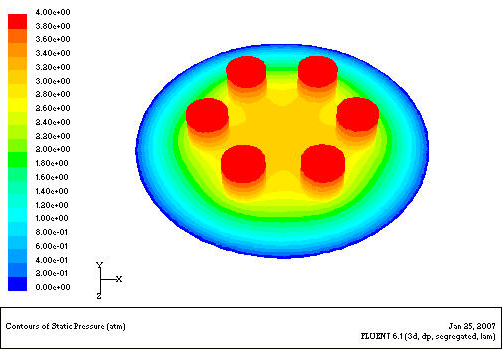
\includegraphics[width=0.8\linewidth]{figures/1.png} %{}内为图片的路径
\figcaptioncneng{局部多孔质圆柱塞半径不同时轴承的压力分布云图} % 图片的中文标题
\label{fig:system} % 正文中通过\ref{fig:system} 引用该图片
\end{figure}

从图~\ref{fig:bearing-pressure}可知，由于节流半径不同，导致节流效果产生很大的不同，其中，半径小的节流效果明显，图~\subref{subfig:bearing-15}对应的压力变化最明显，而图~\subref{subfig:bearing-45}的变化非常小，这导致了气膜内的压力分布产生了很大的不同。从而使承载能力随着半径的增加而得到很大的提高。3. 插图编排:插图之前，文中必须有关于本插图的提示，如“见图1-1”、“如图1-1所示”等。插图与其图题为一个整体，不得拆开排写于两页。插图处的该页空白不够排写该图整体时，则可将其后文字部分提前排写，将图移到次页。3. 插图编排:插图之前，文中必须有关于本插图的提示，如“见图1-1”、“如图1-1所示”等。插图与其图题为一个整体，不得拆开排写于两页。插图处的该页空白不够排写该图整体时，则可将其后文字部分提前排写，将图移到次页。3. 插图编排:插图之前，文中必须有关于本插图的提示，如“见图1-1”、“如图1-1所示”等。插图与其图题为一个整体，不得拆开排写于两页。插图处的该页空白不够排写该图整体时，则可将其后文字部分提前排写，将图移到次页。3. 插图编排:插图之前，文中必须有关于本插图的提示，如“见图1-1”、“如图1-1所示”等。插图与其图题为一个整体，不得拆开排写于两页。插图处的该页空白不够排写该图整体时，则可将其后文字部分提前排写，将图移到次页。

\begin{figure}[htbp]
  \centering
  % 第一行：两个子图并排，[b]底部对齐，[t]顶部对齐
  \begin{subfigure}[t]{0.48\textwidth}
    \centering
    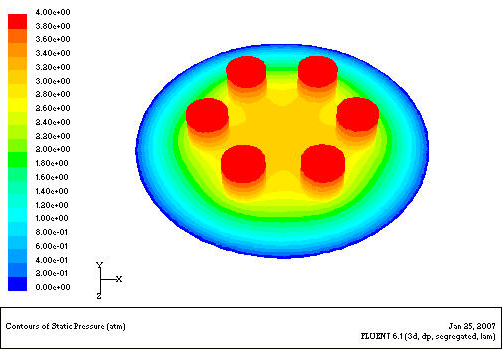
\includegraphics[width=\textwidth]{figures/1.png} % {}内为图片的路径
    \subfigcaptioncneng{$R_3$=1.5mm 时轴承的压力分布云图 时轴承的压力分布云图$R_3$=1.5mm 时轴承的压力分布云图$R_3$=1.5mm 时轴承的压力分布云图。} % 子图标题
    \label{subfig:bearing-15} % 子图标签
  \end{subfigure}
  \hfill
  \begin{subfigure}[t]{0.48\textwidth}
    \centering
    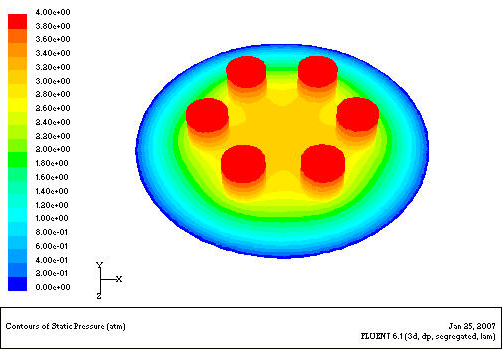
\includegraphics[width=\textwidth]{figures/1.png}
    \subfigcaptioncneng{$R_3$=2.5mm 时轴承的压力分布云图。}
    \label{subfig:bearing-25}
  \end{subfigure}
  \vspace{1em} % 两行之间的间距
  
  % 第二行：两个子图并排
  \begin{subfigure}[b]{0.48\textwidth}
    \centering
    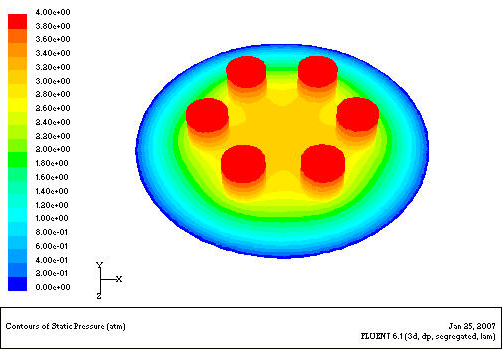
\includegraphics[width=\textwidth]{figures/1.png}
    \subfigcaptioncneng{$R_3$=3.5mm 时轴承的压力分布云图。}
    \label{subfig:bearing-35}
  \end{subfigure}
  \hfill
  \begin{subfigure}[b]{0.48\textwidth}
    \centering
    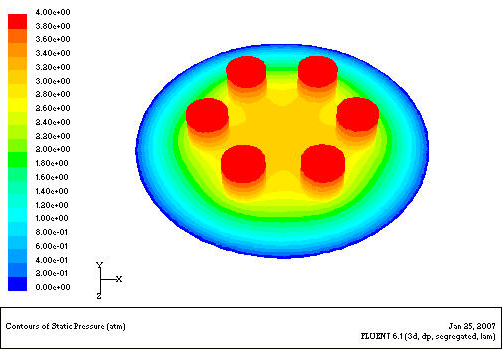
\includegraphics[width=\textwidth]{figures/1.png}
    \subfigcaptioncneng{$R_3$=4.5mm 时轴承的压力分布云图。}
    \label{subfig:bearing-45}
  \end{subfigure}
  
  % 主图标题
  \figcaptioncneng{局部多孔质圆柱塞半径不同时轴承的压力分布云图。} % 主图标题
  \label{fig:bearing-pressure} % 主图的标签
\end{figure}

3. 插图编排:插图之前，文中必须有关于本插图的提示，如“见图1-1”、“如图1-1所示”等。插图与其图题为一个整体，不得拆开排写于两页。插图处的该页空白不够排写该图整体时，则可将其后文字部分提前排写，将图移到次页。3. 插图编排:插图之前，文中必须有关于本插图的提示，如“见图1-1”、“如图1-1所示”等。插图与其图题为一个整体，不得拆开排写于两页。插图处的该页空白不够排写该图整体时，则可将其后文字部分提前排写，将图移到次页。3. 插图编排:插图之前，文中必须有关于本插图的提示，如“见图1-1”、“如图1-1所示”等。插图与其图题为一个整体，不得拆开排写于两页。插图处的该页空白不够排写该图整体时，则可将其后文字部分提前排写，将图移到次页。3. 插图编排:插图之前，文中必须有关于本插图的提示，如“见图1-1”、“如图1-1所示”等。插图与其图题为一个整体，不得拆开排写于两页。插图处的该页空白不够排写该图整体时，则可将其后文字部分提前排写，将图移到次页。